\documentclass{standalone}

\usepackage{tikz}
    \usetikzlibrary{arrows.meta}
    \usetikzlibrary{calc}
    \usetikzlibrary {decorations.pathmorphing}
    % \usetikzlibrary {decorations.pathreplacing}
    % \usetikzlibrary {decorations.shapes}
    \tikzset{st/.style={shape=circle, draw, line width=1mm, inner sep=1mm, }, }
    
\begin{document}
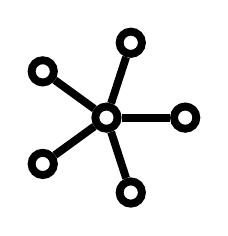
\begin{tikzpicture} %t7
        \node[st,shift={(0,0)}] (k0){};
        \node[st,shift={(72:1)}] (k1){};
        \node[st,shift={(144:1)}] (k2){};
        \node[st,shift={(216:1)}] (k3){};
        \node[st,shift={(288:1)}] (k4){};
        \node[st,shift={(360:1)}] (k5){};
        \path[line width=1mm]
            (k0) edge (k1) edge (k2) edge (k3) edge (k4) edge (k5);
    \end{tikzpicture}
\end{document}